%\documentclass[sigconf, titlepage, twoside]{acmart}
\documentclass[12pt,titlepage, twoside]{article}
%\usepackage{titlesec}

% language stuff
\usepackage{german}           % deutsche Überschriften etc.
\usepackage[utf8]{inputenc} % direkte Einbgabe von Umlauten

% Layout-Einstellungen
\usepackage{parskip}          % Abstand statt Einrückung
\frenchspacing                % no extra space after periods
\usepackage{parskip}          % paragraph gaps instead of indentation
\usepackage{times}            % default font Times
\tolerance=9000               % avoid words across right border

% miscellaneous
\usepackage{graphicx}         % graphics
\usepackage{hhline}           % double lines in tables
\usepackage{amsfonts}         % real numbers etc.
\usepackage[rightcaption]{sidecap} % figure captions on the right (optional)
\usepackage{hyperref}         % for URLs
\usepackage{listings}         % for code samples
\usepackage{fancyhdr}         % for header line
\usepackage{lastpage}         % for last page count

\usepackage{makecell}

\usepackage{xcolor}           % Code highligting

\colorlet{punct}{red!60!black}
\definecolor{background}{HTML}{EEEEEE}
\definecolor{delim}{RGB}{20,105,176}
\definecolor{string}{RGB}{0,0,255}
\colorlet{numb}{magenta!60!black}

\lstdefinelanguage{json}{
    basicstyle=\normalfont\ttfamily,
    %numbers=left,
    %numberstyle=\scriptsize,
    stepnumber=1,
    numbersep=8pt,
    showstringspaces=false,
    breaklines=true,
    frame=lines,
    stringstyle=\ttfamily\color{string},
    %backgroundcolor=\color{background},
    literate=
     *{0}{{{\color{numb}0}}}{1}
      {1}{{{\color{numb}1}}}{1}
      {2}{{{\color{numb}2}}}{1}
      {3}{{{\color{numb}3}}}{1}
      {4}{{{\color{numb}4}}}{1}
      {5}{{{\color{numb}5}}}{1}
      {6}{{{\color{numb}6}}}{1}
      {7}{{{\color{numb}7}}}{1}
      {8}{{{\color{numb}8}}}{1}
      {9}{{{\color{numb}9}}}{1}
      {:}{{{\color{punct}{:}}}}{1}
      {,}{{{\color{punct}{,}}}}{1}
      {\{}{{{\color{delim}{\{}}}}{1}
      {\}}{{{\color{delim}{\}}}}}{1}
      {[}{{{\color{delim}{[}}}}{1}
      {]}{{{\color{delim}{]}}}}{1},
}

% Hier bei Bedarf die Seitenränder einstellen
\usepackage{geometry}
%\geometry{a4paper}
\geometry{a4paper,left=25mm,right=25mm, top=3.5cm, bottom=2.5cm} 

% Kopf- und Fußzeile
\fancyhead{} % clear all header fields
\fancyhead[RO,LE]{\leftmark}

%%%%%%%%%%%%%%%%%%%%%%%%%%%%%%%%%%%%%%%%%%%%%%%%%%%%%%%%%%%%%%
\begin{document}


%-------------------------------------------------------------
\begin{titlepage}
%-------------------------------------------------------------
\begin{center}
{\Large\bf Analyse von Pflanzenwachstum auf Basis von 3D-Punkwolken}\\[3cm]

{\bf Masterarbeit}\\
zur Erlangung des Grades {\em Master of Science}\\[1.5cm]

an der\\
Hochschule Niederrhein\\
Fachbereich Elektrotechnik und Informatik\\
Studiengang {\em Informatik}\\[3cm]

vorgelegt von\\
Jakob Görner\\
1003660\\[3cm]
Datum: \today\\[3cm]

Prüfer: Prof.~Dr.~Regina Pohle-Fröhlich\\
Zweitprüfer: Prof.~Dr.~Christoph Dalitz

\end{center}
\end{titlepage}

\pagestyle{empty}
\cleardoublepage

\newpage


%-------------------------------------------------------------
\section*{Eidesstattliche Erklärung}
%-------------------------------------------------------------
\begin{tabbing}
Name: \hspace{4em}\= Jakob Görner\\
Matrikelnr.: \> 1003660\\
Titel: \> Analyse von Pflanzenwachstum auf Basis von 3D-Punkwolken
\end{tabbing}

Ich versichere durch meine Unterschrift, dass die vorliegende
Arbeit ausschließlich von mir verfasst wurde.
Es wurden keine anderen als die von mir angegebenen Quellen und Hilfsmittel
benutzt.

Die Arbeit besteht aus \pageref{LastPage} Seiten.

\vspace{8ex}
\begin{tabbing}
\underline{\hspace{14em}} \hspace{3em}\= \underline{\hspace{14em}} \\
Mönchengladbach, \today \> Unterschrift
\end{tabbing}

\newpage
%\begin{abstract}
%-------------------------------------------------------------
\section*{Zusammenfassung}
%-------------------------------------------------------------
In dieser Arbeit soll eine Anwendung zum Analysieren von Pflanzen-Wachstum und weiteren Merkmalen des Wachstumsprozesses einer Pflanze erstellt werden. 
Es soll aus einer Reihe Bilder einer Pflanze, die mit einer gängigen Smartphone-Kamera aufgenommen sind, eine Punkwolke erzeugt werden. 
Aus der Punktwolke sollen die Punkte die zur Pflanze gehören extrahiert werden. 
Die extrahierten Punkte werden zur weiteren Analyse in Stamm und Blatt Punkte segmentiert.
Des weiteren sollen Werte wie das Wachstum der Pflanze ermittelt werden. Hierzu müssen mehrere Punktwolken über Zeit miteinander verglichen werden.
Die Anwendung soll mit möglichst wenig Bildern auskommen um den Datentransfer zu minimieren.

\setcounter{page}{1}
%-------------------------------------------------------------
\section*{Abstract}
%-------------------------------------------------------------
Development of an application made to analyse plant growth over time and further characteristics of a plant represented as a point cloud. The point cloud should be generated out of a set of images of the plant, taken with a common smartphone.
The point cloud should be splitted in leave and stem points to count leaves and analyse the stem further. 
Also other characteristics as the hight should be analysed. For this reason multiple point clouds has to be compared over time.
The application should use as few pictures as possible to reduce the amount of transfered data.

%\end{abstract}
\newpage

\pagestyle{plain}
\tableofcontents
\newpage

%-------------------------------------------------------------
% default a), b), c) numbering
\renewcommand{\labelenumi}{\alph{enumi})} 

%=============================================================


\section{Motivation}
%-------------------------------------------------------------
\label{sec:einleitung}
Diese Arbeit wird im Rahmen eines Projekts mit den Universitäten Makerere University (Kampala, Uganda) und Central University of Technology (Bloemfontein, South Africa) durchgeführt.
Im Rahmen dieser Arbeit soll eine Anwendung entstehen, die in den beiden Ländern für Kleinbauern zum Einsatz kommen soll.
Die Anwendung soll mit nicht invasiven Methoden zur Unterstützung bei der selektiven Züchtung eingesetzt werden.
Ziel ist es eine Software zu schaffen die es ermöglicht aus Bildern von Pflanzen 3D Punktwolken (Punktwolken) zu generieren und diese zu analysieren.
Es soll mit der zu entwickelnden Anwendung möglich sein Aussagen über das Wachstum über Zeit, die Entwicklung der Blätter und der Stämme zu treffen. 
Mit diesen Daten sind Analysen möglich die auf das Wachstum einer Pflanze unter bestimmten Bedingungen schließen lassen.
Hierbei gibt es besondere Anforderungen an den Prozess der Datengewinnung und Übertragung. Zum einem muss der Betrieb kostengünstig sein - das betrifft insbesondere den Endverbraucher.
Der Endverbraucher sollte möglichst wenig Datenmengen an den Server, der die Rechenkapazität bereit stellt übertragen muss. Das soll die Kosten auf Seiten des Verbrauchers gering halten.
Desweiteren muss die Datengewinnung mit einem Mobiltelefon oder einer anderen Kamera möglich sein. Spezielle Aufnahmegeräte wie ein LIDAR-Scanner sollten nicht nötig sein.

TODO: Hintergrund der Arbeit. Stichwort Ernährungssicherheit, Ertrags- und Gewinnmargen, Klimaveränderungen

\newpage
\section{Stand der Technik}
%-------------------------------------------------------------
\label{sec:stand}
%Hier müssen Sie beschreiben wie die Situation vor Ihrem Beitrag war.
%Dazu gehören die Vorarbeiten anderer, auf denen Sie aufsetzen, die
%bisher eingesetzte Software oder Hardware und allgemeine
%bekannte Techniken, die in Ihrer Arbeit zum Einsatz kamen.
%
%In diesen Abschnitt gehören alle Aspekte, die zum Verständnis der
%Arbeit erforderlich sind, aber einem mit der Aufgabenstellugn nicht vertrauten
%fachkundigen Leser nicht zwangsweise bekannt sind.

Drei Kernprobleme müssen betrachtet werden die für den Erfolg diese Arbeit gelöst werden müssen. 
Zuerst muss aus einer Menge an Bilder eine Punkwolke generiert werden. Danach muss die Punktwolke Segmentiert werden um den Hintergrund zu entfernen und die einzelnen Teile der Pflanze weiter zu analysieren. 
Zuletzt müssen zwei Punktwolken einer Pflanze zu verschiedenen Zeitpunkten miteinander registriert werden um Aussagen über das Wachstum einer Pflanze treffen zu können.

\subsection{Generierung einer 3D Punkwolke aus Bildern}
\label{sec:stand:pointcloud}

Generell kann man zwischen zwei Methoden der Generierung von Punktwolken unterscheiden, die jeweils verschiedene Verfahren beziehungsweise Techniken anwenden.

Die erste Methode nutzt Hardware wie LIDAR-Scanner \cite{lidar} um Punkwolken direkt zu erzeugen. Es gibt eine Reihe von Sensoren die das ermöglichen. Da der Großteil der Sensoren aus kostengrünen nicht in Frage kommt sei hier nur noch der RGB-D erwähnt. 
Dieser liefert neben den Farbwerten für ein Bild auch noch eine Tiefeninformation für jeden Pixel. In einigen Smartphone-Modellen wird bereits ein solcher Sensor verbaut \cite{rgbd_smartphones}.

Die andere Methode ist Structure from Motion (SfM), bei der die Punktwolke aus Bildern, einer Szene aus verschiedenen Perspektiven, generiert wird. 
Allgemein werden auf den zugrundeliegenden Bildern nach Merkmalen (Feature) gesucht die robust gegen Translation, Rotation, Skalierung und Beleuchtung sind. 
Hier können SIFT \cite{Sift}, ORB \cite{ORB}, BRIEF \cite{BRIEF} oder SURF \cite{SURF} eingesetzt werden.
Wurden die Feature ermittelt müssen korrespondierende Feature zwischen den Bilder ermittelt werden. Das Bild-Paar mit den meisten übereinstimmungen wird als Basis für die Rekonstruktion der 3D-Punkwolke genutzt.
Wurde aus den beiden Bildern eine initiale Punktwolke erstellt, wird diese mit den verbleibenden Bildern angereichert \cite{alouacheevaluation}. 

%Eine der bekanntesten Algorithmen ist SIFT \cite{Sift3D}.
Einige Verfahren benötigen genaue Informationen über die Kamera Position, Ausrichtung und andere Angaben wie die Brennweite der Linse etc. 
andere wiederrum lesen diese Informationen aus den EXIF-Headern der Bildern direkt aus oder schätzen diese \cite{ODM} \cite{schoenberger2016mvs}.

Es wurden in den letzten Jahren große Fortschritte im Bereich Deep Learning, zur Gewinnung von 3D-Punkwolken, gemacht \cite{fan2016point} \cite{tatarchenko2017octree} \cite{wang2018pixel2mesh}. 
Mit diesen Verfahren ist es möglich aus einer minimalen Datenbasis die auch nur aus einem Bild bestehen kann 3D-Punkwolken zu generieren. Was dem Ziel die Datenübertragung zum Server gering zu halten entgegenkommt.
Nachteil der Verfahren ist, dass auf dem Bild nur ein Objekt ohne Hintergrund abgebildet sein darf, oder das zu erkennende Objekt mit einer Binären Maske maskiert werden muss.
Eine Rekonstruktion von komplexen Szenen ist so nicht oder nur mit sehr hohem Aufwand möglich \cite{rs11222644} und wird daher nicht weiter untersucht. 
Der in \cite{rs11222644} vorgestellte Ansatz geht diese Problematik an und soll daher untersucht werden.

%TODO Verfahren auflisten SIFT, RANSAC?, 

\subsection{Segmentierung von 3D-Punkwolken}
\label{sec:stand:segmentierung}

Unter der Segmentierung von 3D-Punktwolken versteht man, dass jedem Punkt ein Label zu zugewiesen wird, welches Auskunft über eine Eigenschaft des Punktes gibt. Im Falle dieser Arbeit sollen Label wie Stamm, Blatt, Blüte oder Frucht vergeben werden.

Bei der Analyse von Pflanzen in Form von 3D Punktwolken gibt es einige nicht gelernte Lösungen \cite{ThreeBasics} \cite{RegionGrowing} die das segmentieren von 3D Punktwolken von Pflanzen in Stiele und Blätter behandeln, 
viele dieser Ansätze haben aber das Problem, dass sie nur unter bestimmten Bedingungen gute Ergebnisse liefern. 
Insbesondere die hohe Qualität der Punktwolken die meist mit einem LIDAR-Scanner oder einem vergleichbaren Gerät erzielt wird, 
kann mit bildbasierten Methoden wie SfM nicht oder nur mit sehr großen Datenmengen und dem damit verbundenen Rechenaufwand erreicht werden. 
Ein weiteres Problem das viele Lösungen haben ist, dass der Hintergrund, also alles was nicht zur Pflanze gehört, manuell entfernt wird, 
oder der Hintegrund so vorbereitet wird das dieser beim erstellen der Punktwolke ignoriert wird und erst auf der freigestellten Pflanze der eigentliche Ansatz ausgeführt wird. 
Um diese Lösungen dennoch in einer voll automatischen Pipeline nutzen zu können muss das freistellen der Pflanzen erst automatisiert werden.
Auch im Bereich Segmentierung wurden große Fortschritte im Bereich Deep Learning auf 3D-Punkwolken gemacht, die mit einer angelernten Netzarchitektur bestimmte Objekte erkennen und Teile davon segmentieren. 
Diese Ansätze können auch auf Pflanzen angewandt werden. Dazu müssen Architekturen wie PointNet\cite{qi2017pointnet}/PointNet++\cite{qi2017pointnet++} oder DGCNN \cite{dgcnn} auf Punktwolken von Pflanzen trainiert werden.  

\subsection{Registrierung von 3D-Punkwolken}
\label{sec:stand:registrierung}

Bei der Registrierung von 3D-Punktwolken probiert man eine Transformationen $T$ zu finden die eine Quell-Punktwolke $S_p$ so transformiert, dass der Abstand $d(S_p,T_p)$ zu einer Ziel-Punktwolke $T_p$ minimiert wird.

Die am weitesten verbreitete Method zur Registrierung von 3D Punktwolken ist Iterative Closest Points (ICP) \cite{icp_org}. ICP basiert auf dem Ansatz das zwei Punktwolken iterativ aneinander angenähert werden.
Dabei wird bei jeder Iteration für jeden Punkt $p_i$ aus der Quellpunkwolke $S_p$ der Punkt aus der Zielpunktwolke gesucht der $p_i$ am nächsten ist. In einem zweiten Schritt wird der Abstand zwischen den korrespondierenden Punkten minimiert.
Zuerst wird für jede Punkwolke das Massezentrum $c_s$ und $c_t$ berechnet und $S_p$ um die Differenz $c_t - c_s$ verschoben. Danach wird mittels Singulärwertzerlegung die Rotation $R$ ermittelt und auf $S_p$ angewandt.
Der Vorgang wird wiederholt bis es zu einer Konvergenz kommt, also $T$ nahezu der Einheitsmatrix $I$ entspricht.

Ein Problem das ICP hat ist, das es auch für lokale Minima konvergiert. Das heißt, das eine initiale Transformation von $S_p$ so gewählt werden muss, so dass der ICP-Durchlauf bei einem globalen Minimum konvergiert.
Ansätze wie global ICP, die mit verschiedenen initialen Transformationen starten existieren sind aber sehr Rechenaufwendig und damit recht langsam.

Des weiteren ist ICP anfällig für Ausreißer. Für diese Problem gibt es allerdings existierende Lösungen \cite{ICP}. Hierbei kommt in der Regel RANSAC \cite{RANSAC} zum Einsatz um Ausreißer bei der Registrierung auszuschließen.
RANSAC basiert auf der Idee ein Model in einer Punktwolke zu suchen und möglichst viele Punkte zu finden die in das Model passen. Initial werden zufällig Punkte gezogen um das Model minimal zu repräsentieren. 
So werden zum Beispiel für ein Linien-Model zwei zufällige Punkte aus der Punktwolke gezogen. Nun werden die Parameter für das Model mit den gezogenen Punkten ermittelt und alle Punkte die nahe genug an dem Model sind mit aufgenommen.
Wenn der Anteil der Punkte die in das Model fallen über einem bestimmten Schwellwert liegen, terminiert der Algorithmus. 
Ansonsten wird der Vorgang solange wiederholt bis eine Parametrisierung gefunden wurde die terminiert oder eine Obergrenze an Iterationen erreicht wurde.
Das Ergebnis des Algorithmus ist auf der einen Seite die gefundene Parametrisierung und auf der anderen Seite eine Unterteilung der Punkte in der Punktwolke in Punkte die in das Model mit gegebener Parametrisierung fallen und in die die nicht in das Model fallen.
Letzteres kann genutzt werden um Punkte bei der Registrierung auszuschließen.

Ein weiteres Problem ist, dass die meisten ICP-Ansätze die Skalierung nicht beachten. Es gibt einige wenige Ansätze für dieses Problem \cite{Ziner2005PointSR}.

Auch für das Registrierung-Problem gibt es Lösungen aus dem Deep-Learning-Bereich, aber auch hier gibt es das Problem, dass es nur wenige Ansätze gibt die mit Skalierung umgehen können.
Bekannt Ansätze sind DCP \cite{Wang_2019_ICCV}, PointNetLK \cite{aoki2019pointnetlk}, RPM-Net \cite{Yew_2020}, DeepGMR \cite{yuan2020deepgmr}, PRNet \cite{wang2019prnet} und PCRNet \cite{sarode2019pcrnet}.

\newpage
\section{Realisierung}
%-------------------------------------------------------------
\label{sec:realisierung}
Es müssen vier Teilprobleme berücksichtigt werden. Zu Beginn muss aus einer Reihe Bilder eine Punktwolke generiert werden. Hauptziel hierbei ist es möglichst wenig Bilder zu benötigen. 
Trotzdem müssen Aspekte wie die Qualität der Punkwolken berücksichtigt werden. 

Ein zweites Problem ist die Registrierung zweier Punktwolken einer Pflanze zu verschiedenen Zeitpunkten um diese Vergleichen zu können. 
Hierbei gilt es die ideale Transformation $T$ bestehend aus Rotation, Skalierung und Translation zu finden um die beiden Punktwolken so realitätsnah wie möglich aneinander aus zu richten.
Es werden drei Ansätze überprüft dieses Problem zu lösen. 
Der erste Ansatz basiert auf der Idee, beim Beginn einer neuen Zeitserie zur Analyse eines Wachstumsprozesses, eine Punktwolke des Hintergrunds zu erstellen und die Punktwolken der einzelnen Zeitpunkte mit diesem Hintegrund zu registrieren. 
So wird ein Verhältnis geschaffen das dem der Realität entspricht.
Der zweite Ansatz basiert darauf das die Registrierung direkt zwischen zwei Zeitpunkten erfolgt. Hierbei kann es zu Abweichungen von der Realität kommen, wenn die Pflanzen skaliert werden müssen für die Registrierung.
Der letzte Ansatz soll überprüfen ob es mittels eines platziertem Objekts möglich ist die skalierung der Punktwolke zu ermitteln und so das Problem beim direkten Vergleich zweier Szenen lösen soll.

TODO: Platziertes Objekt Ansatz umsetzen oder entfernen.

Das dritte Problem ist die Segmentierung der Punktwolke in Stamm, Blätter und Hintergrund. Hier gibt es viele Ansätze dieses Problem zu lösen. Allerdings ist es schwer eine allgemein gültigen Lösung zu finden. 
Ziel ist es daher eine Lösung zu finden die auf möglichst vielen Varianten von Pflanzen funktioniert. 
Das Problem der Segmentierung ist essentiell für die weitere Analyse einer Zeitserien. Ohne die Information welche Punkte zu Stamm und Blättern gehören kann nicht auf die Entwicklung von Blättern und Stielen geschlossen werden.

Zuletzt müssen aus die bisherigen Problemen in geeignete Pipelines zusammengefasst werden und durch einen Server angesteuert werden. Hier muss die Lastverteilung und Datenhaltung beachtet werden.

\subsection{Architektur}
%-------------------------------------------------------------
\label{sec:realisierung:architektur}
%Zwingend erforderlich ist ein Überblick über die Komponenten Ihrer Lösung
%und deren Zusammenspiel. Dazu gehört in der Regel auch ein Diagramm
%der Systemarchitektur.

Die Anwendung soll über eine REST-API angesteuert werden können. Es soll möglich sein eine neue Messreihe anzulegen. Dazu müssen die Bilder für die initiale Punkwolke auf den Server übertragen werden. 
Es soll möglich sein weitere Messpunkte zu einer Messreihe hinzuzufügen. Zu einer Messreihe sollen Auswertungen zur Verfügung gestellt werden. 
Zu jeder Messreihe soll ein Bearbeitungs-Status abgerufen werden können, da die einzelnen Pipelines asynchrone im Hintergrund ausgeführt werden sollen.

TODO: Workflows darstellen. Sequenzdiagramme oder ähnliches.

\subsection{Umsetzung Generierung einer 3D Punktwolke aus Bildern}
%-------------------------------------------------------------
\label{sec:realisierung:implementierung1}
%Dies ist in der Regel nicht nur ein Abschnitt, sondern mehrere Abschnitte
%mit Ihrem Projekt angemessenen Überschriften. Hierhin gehört {\em nicht}
%der Sourcecode Ihrer Lösung, sondern eine textuelle und grafische
%(z.B.~Klassendiagramm) Beschreibung. Bei Quellcode beschränken Sie Sich
%bitte auf kurze, aussagekräftige Ausschnitte.

Die aus der Analyse der verschiedenen Verfahren (siehe Evaluation) ausgewählte Anwendung ODM wird als Docker bereit gestellt. Um den Docker aus zu führen muss eine Ordner-Struktur erstellt werden.
In dieser Ordner-Struktur muss ein Ordner "images" enthalten sein, der die Bilder des Datensatzes, aus dem eine Punktwolke generiert werden soll, enthält.

Ist das Verzeichnis angelegt kann der Docker gestartet werden. Hierbei muss allerdings beachtet werden, dass der Docker mit den selben Rechten wie der User arbeitet. Ansonsten werden per Standarteinstellung Root-Rechte genutzt.
Das führt dazu das auf die erstellten Daten nur noch lesend zugegriffen werden kann, was das Aufräumen erschwert.

\subsection{Umsetzung Registrierung zweier Punktwolken}
%-------------------------------------------------------------
\label{sec:realisierung:implementierung2}

Bei der Umsetzung der Registrierung muss die Besonderheit beachtet werden, dass die Skalierung der Punktwolken nicht bekannt ist und sich unterscheiden. Das heißt die Punkwolken liegen in unterschiedlichen Maasstäben vor.  
Um ein gutes Verfahren zu finden was mit dieser Besonderheit umgehen kann wurden mehrere Ansätze verglichen.

In einem ersten Ansatz wurde versucht ein Pipeline zu erstellen die eine gute Initiale Lösung findet ohne den ganzen Suchraum SO(3) zu durchsuchen.
Die Pipeline sucht zuerst für die Quell- und Ziel-Punktwolke $S$ und $T$ nach der größten Ebene in der Punkwolke und richtet die Punkwolke so aus, dass die gefundene Ebene auf der Ebene liegt, die die x und y Achse bilden.
Des weiteren werden aus beiden Punkwolken nur ein Teilmenge $P_c$ der Punkte in einem Radius $r$ um dem Punkt $c$ der das Zentrum der Masse der Punktwolken repräsentiert entnommen.
Damit soll Rauschen an den Rändern verhindert werden und ein Teil des Hintergrunds soll ausgeblendet werden.
Aus diese Teilmenge werden Subsample gezogen um den Rechenaufwand zu minimieren. In diesem Zustand haben Quell- und Ziel-Punktwolke eine gute initiale Transformation.
Für die zu registrierende Punktwolke wird zunächst mittels SIFT 3D \cite{Sift3D} eine Verbesserung der initiale Transformation gesucht. Danach wird ein ICP-Durchlauf gestartet der auch die Skalierung der Ziel-Punktwolke schätzt.
Um das Ergebnis nach der Schätzung der Skalierung weiter zu verbessern wird noch ein ICP-Durchlauf gestartet - diesmal ohne Schätzung der Skalierung.

Ein weiterer Ansatz ist es DCP so abzuwandeln das statt Translations-Vektor und Rotations-Matrix direkt die ganze Transformations-Matrix geschätzt wird. 
Dazu muss der SVD-Head so angepasst werden das er statt einer $3X3$ Rotations-Matrix $R$ und dem Translations-Vektor $\vec(t)$ die Translations-Matrix $T$ zurück geliefert wird.
Um das zu Erreichen muss die Eingabe der Größe $NX3$ auf eine Eingabe der Größe $NX4$ erweitert werden. Hier kann die Eingabe um einen Vektor mit Einsen erweitert werden.
Das führt dazu das die Singulärwert-Zerlegung von $H$ im SVD-Head nun eine $4X4$ Matrix ist. Die Annahme die wir treffen ist das $H$ als Transformations-Matrix interpretiert werden kann.

In einem letzten Ansatz wird die Skalierung geschätzt in dem ein vorgegebener Bereich an Werten für die Skalierung in einer vorgegebenen Schrittgröße $s$ dursucht wird.
Wieder werden die Quell- und Ziel-Punktwolke an der XY-Achse ausgerichtet und eine Teilmenge $P_c$ um das Zentrum $c$ entnommen wie im ersten Ansatz. Auch werden wieder Subsample gezogen.
In jedem Skalierungs-Schritt wird die Punktwolke mit der aktuellen Skalierung skaliert und danach mit einem Registrierungs-Verfahren registriert.
Um die Ergebnisse der einzelnen Registrierungen zu messen wird der Abstand zwischen der transformierten Quell-Punktwolke und der Ziel-Punktwolke berechnet. 
Der Abstand $d(S,T)$ wird so berechnet, dass für jeden Punkt $p$ aus Punktwolke $T$ der Abstand zum nächsten Punkt in der Punktwolke $S$ berechnet wird.

Man könnte auch den Abstand von allen Punkten in $S$ messen, aber das kann zu Problemen bei kleinen Skalierungen führen, da wenn im extrem Fall die Punktwolke $S$ sehr klein ist alle Punkte in $S$ nahezu keinen Abstand mehr zueinander haben.
Man könnt $S$ also auch durch einen Punkt $p_{S}$ abstrahieren.
Bei der Registrierung muss $S$ nur sehr nah an einen Punkt $p_t$ in $T$ sein sodas gilt $p_t \approx p_S$ und der Abstand zwischen $S$ und $T$ geht gegen $0$. Dadurch werden sehr kleine Skalierung durch dieses Maß bevorzugt.
Nimmt man statt aller Punkte in $S$ alle Punkte in $T$ wird der Fehler in diesem Fall größer als 0 sein, es sei den $T$ ist auch sehr groß.

Mit diesem robustem Maß kann man nun die Güte der einzelnen Skalierungs-Iterationen bewerten und die beste Skalierung mit zugehörigen Transformation für Rotation und Translation finden.
Da die Wahl des Registrierungs-Verfahren offen bleibt wurden hier mehrere Verfahren mit einander verglichen. Es wurden ICP, DCP, PointNetLK und RPM-Net miteinander verglichen.

\subsection{Umsetzung Segmentierung}
%-------------------------------------------------------------
\label{sec:realisierung:implementierung3}

Zur Segmentierung der Pflanzen-Punktwolke in Stamm und Blätter wurde ein Ansatz verfolgt der an den in \cite{ThreeBasics} angelehnt ist, der mittels der Hauptkrümmung eines Punktes ermitteln soll ob es sich um ein Blatt oder einen Stiel handelt. 
Hierbei wird eine einfache Entscheidungsregel $f(x)$ mittels eines Schwellwerts $T_k$ genutzt: Ist die Stärke der Krümmung $k(x)$ des Punktes höher als der Schwellwert handelt es sich um einen Stiel da diese einen größere Krümmung haben als Blätter.
Die Schwierigkeit ist es einen guten Schwellwert und eine gute Kennzahl für die Stärke der Krümmung zu finden.

Die Hauptkrümmung eines Punktes $p_i$ kann über die Normalen des Punktes und der $k$ nächsten Nachbarpunkte $P_i$ berechnet werden.

\begin{equation}
\label{eq:hauptkruemmung:1}
\vec{m}_j = (I - \vec{n}_i \otimes \vec{n}_i ) \cdot \vec{n}_j
\end{equation}

Aus den Abbildungen $\vec{m}_j$ für alle $P_i$ kann die Kovarianzmatrix $C_i$ berechnet werden \ref{eq:hauptkruemmung:2}.

\begin{equation}
\label{eq:hauptkruemmung:2}
C_i = \frac{1}{k} \sum_{j=1}^k{(\vec{m}_j - \vec{\bar{m}}) \otimes (\vec{m}_j - \vec{\bar{m}})}
\end{equation}

Die Hauptkrümmung kann aus den Eigenwerten $0 \leq \lambda_1 \leq \lambda_2 \leq \lambda_3$ von $C_i$ bestimmt werden. $\lambda_3$ ist die stärkste Krümmung und $\lambda_2$ die schwächste Krümmung.

Einige untersuchte Ansätze für eine Funktion $k(p_i)$ sind in \ref{eq:hauptkruemmung:3} zu finden. 

\begin{equation}
\label{eq:hauptkruemmung:3}
\begin{array}{ll}
k_1(p_i) = \lambda_3 \\
k_2(p_i) = \lambda_2 \\
k_3(p_i) = (\lambda_3 + \lambda_2) / 2 
\end{array}{}
\end{equation}

Je höher der Wert der Funktion $f(p_i)$ aus \ref{eq:manuell_classifier} ist desto Wahrscheinlicher gehört ein Punkt zum Stiel einer Pflanze. Ein guter Wert für den Schwellwert $T_k$ muss in Experimenten für die Funktionen $k_1$, $k_2$ und $k_3$ gefunden werden.

\begin{equation}
\label{eq:manuell_classifier}
f(p_i) = \left\{
\begin{array}{ll}
1 & k(p_i) \geq T_k \\
0 & \, \textrm{sonst} \\
\end{array}
\right. 
\end{equation}

In einem weiteren Ansatz wurde eine Implementierung von PointNet auf einem Datensatz von Pflanzen-Punktwolken trainiert um so einen geeigneten Classifier zu trainieren. 
Der Classifier soll für jeden Punkt einer Punktwolke bestehend aus Position und Normalen eine Schätzung liefern was der Punkt repräsentiert. Mögliche Repräsentationen können Stamm, Blatt oder Hintergrund sein.
Weitere denkbare Repräsentationen können die Früchte und Blüten der Pflanzen sein. Wird die Farbe der Punkwolke mit einbezogen, können auch Krankheitsbilder wie vertrocknende Blätter in die Repräsentation eingeschlossen werden.  
Da die Ergebnisse mit PointNet nicht gut genug waren wurde eine verbesserte Version PointNet++ auf dem Datensatz trainiert. Diese wurde mit und ohne Normalen, mit 2 Labeln ohne Hintergrund und mit 3 Labeln mit Hintergrund trainiert.

Nach der Segmentierung wird das Ergebnis noch einmal überarbeitet. Für jedem Punkt $i$ werden die Schätzungen $N_i$ der $k$ ($k=10$) nächsten Nachbarn bestimmt und aus deren Repräsentations-Schätzungen ein Histogramm $H_i$ erzeugt.
Die Schätzung mit dem höchsten Histogramm-Wert wird als neue Schätzung $s_i$ für den Punkt genutzt. Die Berechnungs-Vorschrift ist in Gleichung \ref{eq:improve_score} zu finden. 
Dieser Vorgang wird für alle Punkte solange wiederholt bis es bei den Punkten zu keinen Änderungen mehr kommt oder eine maximale Iterations-Obergrenze erreicht wird.

\begin{equation}
\label{eq:improve_score}
\begin{array}{l}
L =  \{0,1,2\}\\
w(x) = \left\{
\begin{array}{ll}
0,5 & x = 2 \\
1 & \, \textrm{sonst} 
\end{array}
\right.\\ 
H_i(x) = \sum_{j=0}^{k}{(w(x) | N_{ij} = x)}\\
x \in L\\
s_i = argmax_x(H_i(x))
\end{array}
\end{equation}

\subsection{Umsetzung Server}
%-------------------------------------------------------------
\label{sec:realisierung:implementierung4}

Der Server ist mit dem Python-Framework Flask erstellt. Flask bietet eine Schlanke API um neue REST-Endpunkte zu erstellen und Daten vom Client anzunehmen. 

Ein Hintergrund-Prozess führt die einzelnen Jobs aus und sorgt für den Lastausgleich. Die Anfragen an den Server werden asynchron verarbeitet. 
Jede Anfrage wird in die Job-Queue eingeordnet. Diese wird vom Hintergrund-Prozess abgearbeitet.
Einzige Ausnahme bildet hier das Speichern der Bilder. Die Bilder müssen synchrone zum Request auf der Platte persistiert werden, da Flask die Datei-Streams nach dem Lebenszyklus eines Requests schließt.

Beim Start des Servers wird neben dem Hintergrund-Prozess der aktuelle Stand der Datenhaltung eingelesen und der Status des Servers aufgebaut. 
Bei der Datenhaltung wurde auf eine Datenbank verzichtet, da die meisten Daten als Blob vorliegen und daher nicht geeignet für ein relationales Datenbank-Modell sind. 
Die Daten werden direkt auf der Festplatte des Host-Systems abgelegt.
Des weiteren werden zwei Instanzen von PointNet++ gestartet. Eine für die Segmentierung des Hintergrundes und einer für die Segmentierung der Pflanze.

Der Server bietet folgende Schnittstellen:

\textbf{GET /listings/\{Messreihe\}}

Dient dazu zu einer Messreihe den aktuellen Status abzuholen. Der Status der Messreihe setzt sich aus den einzelnen Pipeline-Status zusammen.

\textbf{PUT /results/\{Messreihe\}/\{Zeitstempel\}}

Dient dazu zu einem Zeitpunkt einer Messreihe die ermittelten Werte wie Anzahl Blätter oder Volumen abzuholen.

\textbf{POST /data/\{Messreihe\}/\{Zeitstempel\}}

Dient dazu neue Datensätze hinzu zu fügen. Es muss eine Sammlung von Bildern einer Pflanze mit geliefert werden. 
Wird der Endpunkt angesprochen werden die Bilder gespeichert und die Pipeline zum generieren der Punktwolke in die Job-Queue hinzugefügt.
Wird als Zeitstempel \"background\" angegeben wird dieser Datensatz als Hintergrund für die derzeitige Messreihe interpretiert.

\textbf{PUT /data/\{Messreihe\}/\{Zeitstempel\}}

Dient dazu Pipelines für einen Zeitstempel einer Messreihe zu starten. Hierzu wird im Payload des Request an den Server eine JSON-Datei übermittelt welches eine Liste der Pipelines enthält (Beispiel siehe Listing \ref{listing:example:payload}).
Die spezifizierten Pipelines werden, in der angegebene Reihenfolge, der Job-Queue hinzugefügt.
\\

\begin{lstlisting}[language=json, caption={Beispiel Payload zum starten einer Pipeline}, captionpos=b, label=listing:example:payload]
{
    "jobs" : [
        {
            "jobName" : "SegmentBackground",
            "jobParameter" : {}
        }
    ]
}
\end{lstlisting}

Es stehen folgende Pipelines zur Verfügung:

\begin{itemize}
\item Punkwolke generieren
\item In Shapnet-Format überführen
\item Entfernung des Hintergrundes
\item Segmentierung Pflanze
\item Blatt/Stamm Trennung
\item Blätter zählen
\item In Registrierungs-Format überführen
\item Hintergrund-Registrierung
\item Größen berechnen
\end{itemize}

Die Pipeline Punktwolke generieren wird mit dem Anlegen eines neuen Zeitstempels gestartet. Es wird aus den hoch geladenen Bildern eine Punktwolke generiert.

\subsection{Umsetzung Pipelines}
%-------------------------------------------------------------
\label{sec:realisierung:implementierung5}

\textbf{Punkwolke generieren}

Die Punktwolke wird auf Basis der hoch geladenen Bilder zu einem Zeitstempel generiert. Beim Anlegen eines neuen Zeitstempels wird die Pipeline automatisch gestartet, kann aber auch manuell neu gestartet werden.

\textbf{In Shapnet-Format überführen}

%TODO: Überdenken ob Shapent-Format der richtige Name ist oder ob Segmentierungs-Format nicht zutreffender ist.

Diese Pipeline überführt die Punktwolke in das Shapenet-Format. Die Punktwolke muss in diesem Format vorliegen um die beiden Segmentierungs-Pipelines nutzen zu können.
Bevor die Punktwolke in das Shapenet-Format überführt wird können zwei optionale Schritte durchgeführt werden.
Bei der Hintegrund-Segmentierung wird die Punktwolke mittels der größten in der Punktwolke zu findenden Ebene an der XY-Ebene ausgerichtet.
Bei der Pflanzen-Segmentierung werden alle als Hintergrund gelabelten Punkte entfernt. Danach beginnt die eigentliche Überführung in das Shapenet-Format.
Zuerst wird die Punktwolke so verschoben, dass die Bounding-Box im Koordinaten-Ursprung beginnt und sich auf den positiven Bereich der Achsen erstreckt.
Danach wird die Punktwolke in der Form normiert, dass sich alle Punkte der Punktwolke zwischen den Punkten $(0,0,0)$ und $(1,1,1)$ befinden.
Zuletzt werden $n=16384$ Punkte aus der Punktwolke zufällig gezogen, wobei die Punkte nicht zurück gelegt werden.

\textbf{Entfernung des Hintergrundes}

Die im Shapenet-Format vorliegende Punktwolke wird mit der Instanz von PointNet++ für die Hintegrund-Segmentierung segmentiert. Das Ergebnis wird im Speicher des Host-Systems abgelget.
Da die Segmentierung etwas verrauscht ist wird das Ergebniss mit einem nächste Nachbarn Vote verbessert.
Im Anschluss wir das Ergebnis auf die original Punktwolke übertragen, da sonst zu wenig Punkte für die Segmenetierung der Pflanze übrig bleiben.
Auch wird der Hintegrund entfernt und aus den verbleibenden Punkten, die nun nur noch Pflanzen-Punkte enthalten wieder eine Punktwolke im Shapenet-Format erstellt.

\textbf{Segmentierung Pflanze}

Auf dem Ergebniss der Hintergrund-Entfernung wird PointNet++ zur Segmentierung der Pflanze gestartet. Auch hier wird das Ergebnis im Speicher des Host-Systems abgegelegt. 
Auch hier wird das Segmentierungs-Ergebniss wie bei der Hintergrundentfernung verbessert.

\textbf{Blatt/Stamm Trennung}

Die Punktwolke die die segmentierte Pflanze enthält wird in zwei Punktwolken aufgeteilt. 
Wobei die eine Punktwolke nur noch Punkte enthält die Blätter repräsentieren und eine die entsprechend nur noch Punkte enthält die Stiele repräsentieren.

\textbf{Blätter zählen}

Die Punktwolke $P$ die die Blätter enthält wird nun mit einer 3D Interpretation des Flood-Fill-Algoritmus untersucht. Hierbei wird ein zufälliger Punkt in der Punkwolke gewählt und in die Menge $Q$ aufgenommen.
Nun wird solange bis $Q$ keine Punkte mehr enhält ein Punkt $p$ aus $Q$ entnommen und mittels nächster Nachbarn-Suche im Radius $r$ nach weiteren Punkten in der Nähe gesucht. Gefundene Punkte werden in $Q$ aufgenommen.
Der Punkt $p$ wird danach in eine Menge $B$ aufgenommen. Ist $Q$ leer wird die Menge $B$ aus $P$ entfernt und der Blatt-Zählstand um eins erhöht. 
Der Vorgang wird so lange wiederholt, bis keine Punkte mehr in $P$ enthalten sind.

\textbf{In Registrierungs-Format überführen}

Zuerst wird die Punktwolke wieder anhand der größten Ebene die in der Punktwolke zu finden ist an der XY-Ebene ausgerichtet.
Danach wird um das Zentrum der Punktwolke ein Ausschnitt entnommen. 
Im folgenden wird die Punktwolke wie beim Shapenet Format normiert und es werden zufällig 1024 Punkte aus der Punktwolke gezogen.

\textbf{Hintergrund-Registrierung}

Um einen Zeitstempel $t$ einer Messung mit dem Hintergrund der Messreihe zu registrieren muss sowohl die Punktwolke $P_t$ für den Zeitstempel $t$ als auch die Punktwolke für den Hintegrund im Registrierungs-Format vorliegen.
Ist das gegeben kann die Registrierung gestartet werden. Hierbei wird ein Skalierungs-Faktor $s$ und eine Transformation $T$ ermittelt. 
Das Registrierungs-Ergebnis der Punktwolke $P_t$ kann dann mit der Formel $P_{Registration} = (P_t \cdot s) \cdot T$ ermittelt werden. Wobei beachtet werden muss, dass erst die Skalierung und dann die Transformation angwandt wird.

\textbf{Größen berechnen}

Ist die Punktwolke $P_t$ zum Zeitstempel $t$ mit dem Hintegrund registriert, können die Größen Höhe und Volumen berechnet werden. Diese sind leicht zu ermitteln. 
Die Höhe kann über den höchsten z-Wert der Punkte in $P_t$ ermittelt werden. Um das Volumen zu berechnen, muss für $P_t$ die Länge $l$, Breite $b$ und Höhe $h$ ermittelt werden. 
Das Volumen $v$ lässt sich dann folgendermaßen berechnen: $v = h \cdot b \cdot l$.

TODO: Formeln für l,b und h

Ist die Höhe für den vorherigen Zeitstempel $t-1$ auch bekannt, kann das relative Wachstum seit dem letzten Zeitpunkt ermittelt werden.

\newpage
\section{Ergebnisse}
%-------------------------------------------------------------
\label{sec:ergebnisse}
%Hierhin gehört eine Beschreibung der von Ihnen durchgeführten Tests zur
%Verifikation bzw.~Qualitätssicherung Ihrer Lösung. Wenn Sie Messungen
%durchgeführt haben, so stellen Sie die Ergebnisse hier in Tabellen und
%Diagrammen dar.
%
%Auch die Diskussion der Messergebnisse oder der Besonderheiten der
%Testergebnisse gehört hierher.

\subsection{Vergleich von Verfahren zur Generierung von 3D-Punktwolken auf Basis von Bildern}

Um eine geeignete Software zur Generierung von 3D-Punktwolken auszuwählen muss erst entschieden werden nach welchen Gütekriterien verschiedene Verfahren betrachtet werden sollen und wie wichtig diese sind.
Bei dieser Arbeit ist die nötige Anzahl der Bilder die zur Generierung einer Punktwolke mit genug Information nötig sind das wichtigste Kriterium.
Um dieses Kriterium zu messen muss ein Goldstandart von der fotografierten Szene als 3D-Punktwolke erstellt werden, mit dem Verglichen werden kann.
Dieser Goldstandart kann erstellt werden, indem alle Fotografien genutzt werden die zur Verfügung stehen und damit alle Verfahren eine Punktwolke erstellen lassen. 
Unter den erstellten Punktwolken kann die ausgesucht werden die die Szene am besten repräsentiert. 
Das trifft auf die Punkwolke zu die den höchsten Detail-Grad hat und möglichst wenig Fehler, wie fehlende Teile der Szene oder Rauschen enthält.
Die so erstellte Szene sollte nachbearbeitet werden um etwaige Fehler wie Rauschen manuell zu entfernen.
Weitere Maße um die Güte des Goldstandarts zu bewerten ist die Anzahl der Punkte in der Wolke oder die Dichte der Punkte in der normalisierten Punktwolke.

Nun kann mit wenigeren Bildern aus dem selben Datensatz ein weitere Punktwolke generiert werden und die Distanz der Punkte der Goldstandart-Punktwolke zum jeweils nächsten Punkt der erstellten Punktwolke gemessen werden.
Die Summe dieser Abstände kann als Fehlermaß genutzt werden. Bei der Berechnung der Abstände muss beachtet werden, dass die Punkwolken mit dem Goldstandart registriert ist.

Ein weiterer Punkt bei der Bewertung des Verfahrens zur Generierung von 3D Punktwolken ist die Zeit die benötigt wird die Punkwolke zu generieren.

TODO: Verfahren vergleich.

TODO: Bilder für einzelne Verfahren

\subsection{Vergleich von Verfahren zur Registrierung 3D-Punkwolken}

In einem ersten Schritt wurden verschiedene Lösungen aus dem Deep-Learning Bereich miteinander Verglichen. 
Es wird die Distanz zwischen transformierter Quell-Punktwolke und Ziel-Punktwolke wie im Abschnitt \ref{sec:realisierung:implementierung2} beschrieben gemessen. Neben der Distanz berichten wir über den bei der Evaluation gemessenen Loss.
Die einzelnen Verfahren sind alle in dem Python-Paket "learning3d" implementiert und nutzen die selbe Datenbasis ModelNet40 für das Training und sind somit gut vergleichbar. Für DCP und RPM-Net wurden das vortrainierte Model vom Author des Pakets genutzt.
PointNetLK musste trainiert werden und wurde mit den empfohlenen Angaben des Authors trainiert. Die Evaluation wurde drei mal mit zufälligen Daten wiederholt und aus den drei Durchläufen die Mittelwerte für die ermittelten Werten gebildet.
Die Ergebnisse sind in Tabelle \ref{tab:registration:deeplearn:compare} zu finden.

\begin{table}
\begin{center}
\begin{tabular}{|l || c | c | c | } 
    \hline
     & DCP & RPM-Net & PointNetLK \\  
    \hline
    \hline
    Distanz & $0,0292$ & $0,0663$& $0,026$\\
    \hline
    Loss & $0,922$& $0,061$& $0,111$\\
    \hline
\end{tabular}
\end{center}
\caption{Vergleich von Registrierungs-Verfahren auf ModelNet40. Distanz und Loss sind jeweils Mittelwerte über alle Datensätze in der Iteration.}
\label{tab:registration:deeplearn:compare}
\end{table}

In einem zweiten Schritt wurden die Verfahren auf konkreten Beispielen der Problemstellung getestet. 

TODO: Tabelle mit Vergleich auf echten Daten für DCP RPM-Net PointNetLK ICP und RICP.

TODO: Erkenntniss aus dem Vergleich. Ggf Bilder von den Ergebnissen.

\subsection{Vergleich von Verfahren zur Segmentierung von Pflanzen auf 3D-Punkwolken}

TODO: Handcrafted Classifier mit PointNet++ vergleichen. Erkenntnis das Handcrafted Classifier auf Grund der ungenauen Punkte nicht funktioniert.

\textbf{Datenbasis für das Training von PointNet++}

Als Datenbasis für das Training von PointNet++ wurden 144 handgelabelte Punkwolken von verschiedenen Pflanzen gewählt. Darunter sind Tomaten, Mais, Paprika, Avocado, Bananen und weitere nicht bekannte Sorten. 
Da diese Datenbasis für das Training eines Neuronalen Netz recht klein ist wurde aus jeder einzelnen Punktwolke bis zu 20 Subsample erstellt. Diese wurden so erstellt, dass zufällig $n$ Punkte aus einer Punktwolke gezogen und entfernt wurden.
Des weiteren sind die Daten so aufbereitet das der Boden der Punktwolke an der XY-Ebene ausgerichtet ist und der Stiel bei geradem Wachstum Richtung z-Achse zeigt. Des weiteren sind die Punkte in der Punktwolke auf 1 normiert. 
Das heißt sie liegen in dem Raum den die beiden Punkte $(0,0,0)$ und $(1,1,1)$ aufspannen. Die Daten werden in einem Verhältnis 80 zu 10 zu 10 in Trainings-, Test- und Evaluations-Datensatz aufgeteilt.

\textbf{Vergleich Training mit und ohne Hintergrund}

TODO: Vergleich Training mit/ohne Hintergrund. Mit Hintergrund -> lohnt es sich nur das Zentrum zu betrachten?

\begin{figure}
    \centering
    \begin{minipage}{0.475\textwidth}
        \centering
        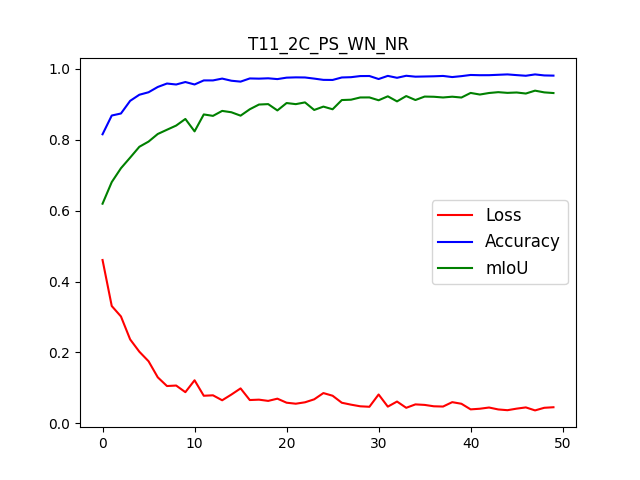
\includegraphics[width=1.0\textwidth]{./Images/T11_2C_PS_WN_NR.png}
        \caption{PointNet++ Trainings-Ergebnisse pro Epoche mit 2 Klassen und Normalisierung ohne zufällige Rotationen}
        \label{fig:T11_2C_PS_WN_NR}
    \end{minipage}\hfill
    \begin{minipage}{0.475\textwidth}
        \centering
        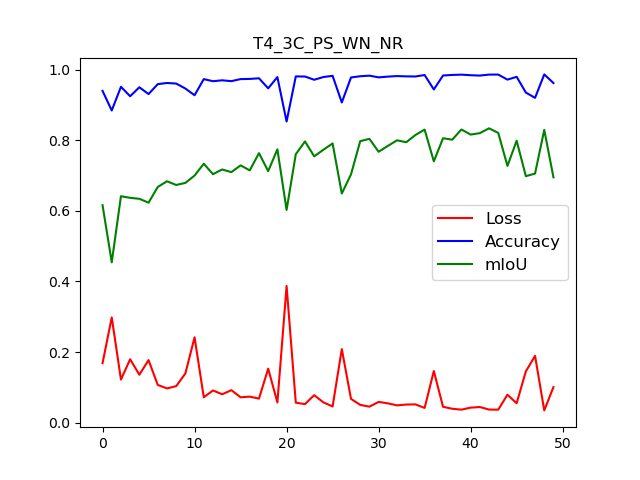
\includegraphics[width=1.0\textwidth]{./Images/T4_3C_PS_WN_NR.png}
        \caption{PointNet++ Trainings-Ergebnisse pro Epoche mit 3 Klassen und Normalisierung ohne zufällige Rotationen}
        \label{fig:T4_3C_PS_WN_NR}
    \end{minipage}
\end{figure}

\textbf{Vergleich Training mit und ohne Normalen}

TODO: Vergleich Training mit/ohne Normalen

\textbf{Vergleich Training mit und ohne Normalisierung}  (Einsatz von nicht normalisierten Punkten trotz Normalisierung im Training möglich?)

Es soll Überprüft werden ob PointNet++ mit oder ohne Normaliserung bessere Ergebnisse liefert. 
Des weiteren soll geprüft werden, ob auch nicht normaliserte Eingabe-Daten gute Segmentierungs-Ergebnisse liefern wenn PointNet++ mit normaliserten Daten trainiert wurde.
Dieser Vergleich wird aufgestellt, da die Punkwolken für die Segmentierung auf eine bestimmte Anzahl Punkte reduziert werden und das Ergebniss - zumindest bei der Hintergrund-Segmentierung - zurück auf die vollständige Punktwolke übertragen werden muss.
%Dafür darf die reduzierte Punktwolke ihre Position nicht ändern. Um das zu gewährleisten muss die Normalisierung die PointNet++ ausführt verhindert oder umgekehrt werden. 
Muss die Punktwolke nicht normalisert werden, kann das Ergebniss direkt auf die vollständige Punktwolke übertragen werden. 
Im Falle einer Normaliserung müsste diese erst umgekehrt werden, aber diese Information wird von PointNet++ nicht zur Verfügung gestellt und müsste ermittelt werden.
Alternativ dazu könnten auch die Ergebnisse von der normalisierten Punktwolke auf die nicht normaliserte Punktwolke übertragen werden, was aber mit mehr Rechenaufwand verbunden ist.

Wird die Normalisierung komplett verhindert, kann das Auswirkungen auf die Güte der Ergebnisse der Segmentierung haben.

\begin{table}
    \begin{center}
    \begin{tabular}{|l || c | c || c | c | } 
        \hline
         & \thead{t4 mit \\ normalisiert Daten}  & \thead{t4 mit \\ nicht normalisiert Daten} & \thead{t11 mit \\ normalisiert Daten} & \thead{t11 mit \\ nicht normalisiert Daten}  \\  
        \hline
        \hline
        Loss & $0,038$ & $0,175$& $-$& $-$\\
        \hline
        Genauigkeit & $0,986$& $0,946$& $-$& $-$\\
        \hline
        IoU & $0,84$& $0,684$& $-$& $-$\\
        \hline
    \end{tabular}
    \end{center}
    \caption{Vergleich von Evaluations-Ergebnissen von den mit normaliserten Daten trainierten Netzen t4 (mit Hintergrund) und t11(ohne Hintergrund) mit jeweils normalisierten und nicht normaliserten Daten.}
    \label{tab:registration:deeplearn:compare}
\end{table}

In Tabelle \ref{tab:registration:deeplearn:compare} sind die Ergebnisse der Evaluation von PointNet++ auf nicht normaliserten Daten nach dem Training mit normaliserten Daten zu sehen.
Da die Ergebnisse sich stark verschlechtern, wenn die Daten nicht normalisiert werden wird PointNet++ ohne Normalisierung erneut trainiert. 
Die Ergebnisse für das erneute Training sind in Abbildung \ref{fig:T6_2C_PS_NN_NR} für zwei Klassen und in Abbildung \ref{fig:T7_3C_PS_NN_NR} für drei Klassen zu sehen.

\begin{figure}
    \centering
    \begin{minipage}{0.475\textwidth}
        \centering
        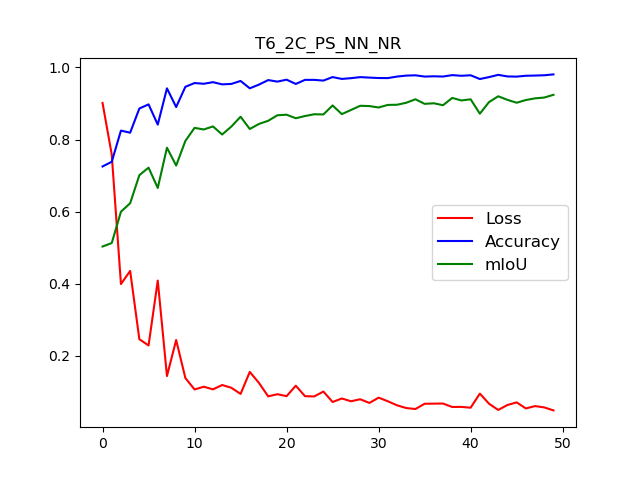
\includegraphics[width=1.0\textwidth]{./Images/T6_2C_PS_NN_NR.png}
        \caption{PointNet++ Trainings-Ergebnisse pro Epoche mit 2 Klassen, ohne Normalisierung und ohne zufällige Rotationen }
        \label{fig:T6_2C_PS_NN_NR}
    \end{minipage}\hfill
    \begin{minipage}{0.475\textwidth}
        \centering
        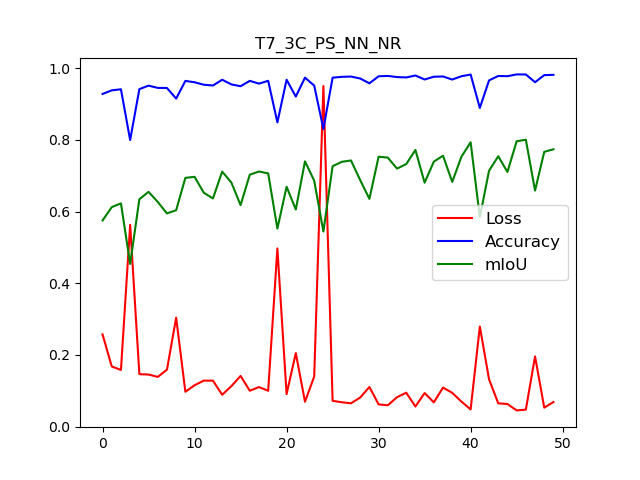
\includegraphics[width=1.0\textwidth]{./Images/T7_3C_PS_NN_NR.png}
        \caption{PointNet++ Trainings-Ergebnisse pro Epoche mit 3 Klassen, ohne Normalisierung und ohne zufällige Rotationen}
        \label{fig:T7_3C_PS_NN_NR}
    \end{minipage}
\end{figure}

Gegenüber dem Training mit Normalisierung ist das Training ohne Normalisierung etwas schlechter. Insbesondere für das Netz mit drei Klassen haben die Ausreißer für Loss-, Accuracy- und IoU-Werte zugenommen.
Das führt zu dem Schluss, dass PointNet++ mit Normalisierung genutzt werden sollt und der zusätzliche Rechenaufwand zum übertragen der Ergebnisse auf die vollständige Punktwolke in kauf genommen werden sollt.

\textbf{Vergleich Training mit und ohne zufällige Rotationen}

Die Tests des Servers haben gezeigt, das es bei der Segmentierung der freigestellten Pflanzen zu starken Fehlern kommt, wenn diese rotiert sind. 
Das hat zu der Erkenntnis geführt, dass PointNet++ anfällig für die Ausrichtung von Punktwolken ist. 
Aus diesem Grund wurde das Training für das zwei und drei Klassen-Netz mit zufälligen Rotationen wiederholt um ein Robustheit gegen Rotationen anzutrainieren.
Die Ergebnisse für zwei Klassen-Netz ist in Abbildung ~\ref{fig:10_2C_PS_WN_RR} zu sehen. Die Ergebnisse für das 3 Klassen-Netz in Abbildung ~\ref{fig:9_3C_PS_WN_RR}. 
Beim Training von dem Netz mit drei Klassen sind starke Ausreißer in den Loss-Werten zu erkennen die sich auch in der Accuracy und dem IoU wiederspiegeln.
Diese Beobachtung kann man bei dem anderen Netz nur in wesentlich kleinerem Ausmaß feststellen. Dennoch sind die Ergebnisse wesentlich schlechter für das Training mit zufälligen Rotationen als das Training ohne.
Im Einsatz sollt also bei der Entfernung des Hintergrundes darauf geachtet werden, dass dieser zumindest grob an der XY-Ebene Ausgerichtet ist.

\begin{figure}
    \centering
    \begin{minipage}{0.475\textwidth}
        \centering
        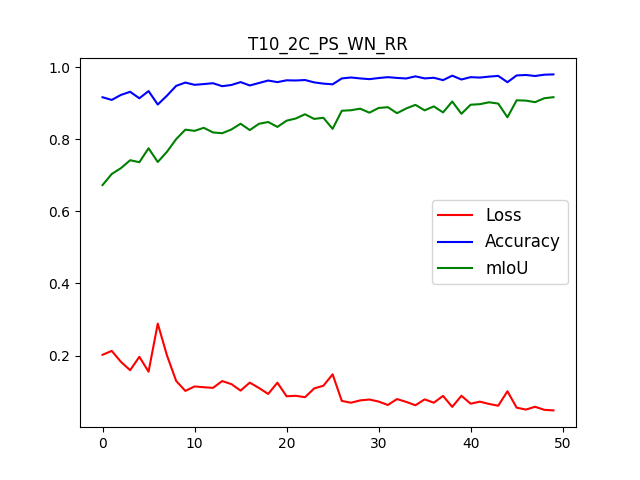
\includegraphics[width=1.0\textwidth]{./Images/10_2C_PS_WN_RR.png}
        \caption{PointNet++ Trainings-Ergebnisse pro Epoche mit 2 Klassen, mit Normalisierung und zufälliger Rotationen}
        \label{fig:10_2C_PS_WN_RR}
    \end{minipage}\hfill
    \begin{minipage}{0.475\textwidth}
        \centering
        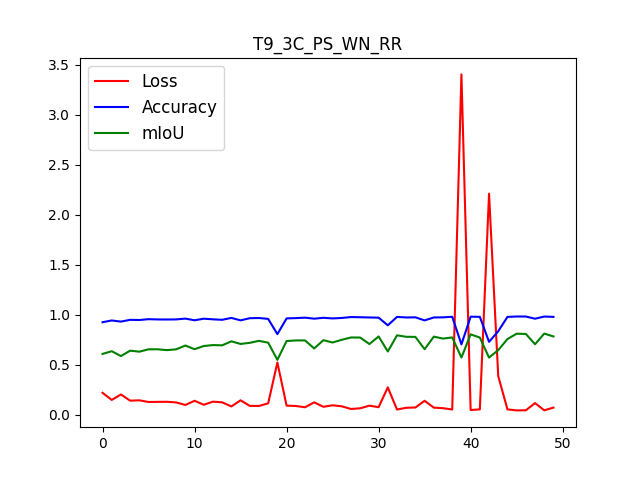
\includegraphics[width=1.0\textwidth]{./Images/9_3C_PS_WN_RR.png}
        \caption{PointNet++ Trainings-Ergebnisse pro Epoche mit 3 Klassen, mit Normalisierung und zufälliger Rotationen}
        \label{fig:9_3C_PS_WN_RR}
    \end{minipage}
\end{figure}

TODO: Bilder von fehlgeschlagener Segmentierung einfügen

\newpage
\section{Fazit und Ausblick}
%-------------------------------------------------------------
\label{sec:fazit}
%Am Ende der Arbeit muss ein Fazit dessen was geleistet wurde
%und wie es weitergehen kann. Dazu gehört auch wie der aktuelle
%Stand Ihrer Implementierung ist: ist Ihre Lösung z.B. bereits
%produktiv im Einsatz? Welche wesentlichen Punkte müssen noch
%umgesetzt werden?
%
%Insbesondere müssen hier die Schwachpunkte
%Ihrer Lösung erwähnt werden, also was Sie anders machen würden,
%wenn Sie dieselbe Aufgabe noch einmal bekämen. Auch nicht gelöste
%oder sich im Laufe der Arbeit neu ergebene Fragen müssen hier zur
%Sprache kommen.

\textbf{Generierung der Punkwolken}

Die Generierung von Punktwolken mit ODM liefert zwar gute Ergebnisse und ist vergleichsweise schnell. Allerdings ist es dennoch die Komponente die am meisten Laufzeit in Anspruch nimmt.
Da keine Geo-Informationen zu den Bilder vorliegen, kann die GPU von ODM nicht eingesetzt werden. An der Stelle könnte ODM erweitert werden und die alternative Implementierung die ohne Geo-Informationen auskommt könnte parallelisiert werden.

Sollte sich in Zukunft bei Smartphones eine RGB-D Kamera als Standart etablieren, könnte diese Technologie genutzt werden um eine schnelle Generierung der Punktwolken zu ermöglichen.

Ein weiterer Ansatz der Untersucht werden könnte ist die Generierung von Punktwolken mit Neuronalen Netzen. Hier gibt es einige interessante Ansätze die im Rahmen dieser Arbeit nicht untersucht wurden. 

\textbf{Registrierung}

Die Ergebnisse der Registrierung sind zwar für den Zweck ausreichend, aber könnten zuverlässiger und genauer sein. Insbesondere die nicht bekannte Skalierung bereitet Probleme.

Bei der Datengewinnung könnte zu den Bildern auch eine GPS-Position ermittelt werden und so Punktwolken mit gleichem Maßstab erstellt werden. Das würde die Registrierung erleichtern, da die Skalierung nicht mehr geschätzt werden müsste.

Ein weiterer Ansatz der in dieser Arbeit nicht verfolgt wurde ist ScaleLK.

\textbf{Segmentierung}

Die Segmentierung ist für die Hintergrundentfernung noch nicht gut genug. Hier könnte probiert werden mit einem größerem Datensatz zu trainieren oder mehr Punkte während des Trainings zu nutzen.

Die Segmentierung der Pflanze kann erweitert werden um zusätzliche Informationen über eine Pflanze zu erhalten. Zum Beispiel können neben Blättern und Stielen auch Blüten und Früchte erkannt werden, was für die Analyse des Ertrags einer Fruchtfolge genutz werden könnte.
Um das zu bewerkstelligen muss für jedes Merkmal ein weiters Label hinzugefügt werden und die Datenbasis, die für das Training genutzt wird, um Punktwolken erweitert werden die diese Merkmale auch beinhalten.

%Weitere Analyse der Daten

\newpage
% Literaturverzeichnis
%-------------------------------------------------------------
\addcontentsline{toc}{section}{Literatur}

\bibliographystyle{ieeetr}
\bibliography{./bibleografie.bib}

\end{document}